% ============================================================
\chapter{Introduction aux Bases de Donn\'ees Relationnelles}
\label{ch:introduction}
% ============================================================

En 1970, Edgar F.\ Codd, chercheur chez IBM, publie un article qui va
r\'evolutionner l'informatique~: \emph{A Relational Model of Data for Large
Shared Data Banks}. Son id\'ee~: organiser les donn\'ees dans des
\emph{tables} reli\'ees par des op\'erations alg\'ebriques pr\'ecises, en
s\'eparant radicalement la mani\`ere dont les donn\'ees sont stock\'ees
physiquement de la mani\`ere dont on les interroge logiquement. IBM, ironie
de l'histoire, met des ann\'ees \`a impl\'ementer les id\'ees de son propre
chercheur --- c'est un groupe de Berkeley, men\'e par Michael Stonebraker,
qui cr\'ee le premier syst\`eme relationnel pratique. Aujourd'hui, les bases
de donn\'ees relationnelles stockent l'essentiel de l'information mondiale.

% ------------------------------------------------------------
\section{Qu'est-ce qu'une base de donn\'ees ?}
% ------------------------------------------------------------

Commen\c{c}ons par la question la plus fondamentale.

\begin{definition}[Base de donn\'ees]
Une \emph{base de donn\'ees} est une collection organis\'ee de donn\'ees
structur\'ees, stock\'ees de mani\`ere persistante et accessibles
par plusieurs utilisateurs et applications de fa\c{c}on contr\^ol\'ee.
\end{definition}

Contrairement \`a un simple fichier (CSV, texte), une base de donn\'ees offre~:
\begin{itemize}
    \item \textbf{Persistance} --- les donn\'ees survivent \`a l'arr\^et du programme.
    \item \textbf{Partage} --- plusieurs utilisateurs acc\`edent simultan\'ement aux donn\'ees.
    \item \textbf{Int\'egrit\'e} --- des contraintes garantissent la coh\'erence des donn\'ees.
    \item \textbf{S\'ecurit\'e} --- des m\'ecanismes de contr\^ole d'acc\`es prot\`egent les donn\'ees.
    \item \textbf{Interrogation efficace} --- un langage d\'eclaratif (SQL) permet de
          poser des questions complexes sans d\'ecrire le \og comment \fg.
\end{itemize}

\begin{exemple}
Consid\'erons un syst\`eme de gestion d'une universit\'e. Sans base de donn\'ees,
on pourrait stocker les \'etudiants dans un fichier CSV~:
\begin{verbatim}
1,Bernard,Alice,2004-03-15,Info
2,Petit,Bob,2003-11-22,Info
\end{verbatim}
Probl\`emes~: pas de v\'erification de type, pas de cl\'e \'etrang\`ere, pas d'acc\`es
concurrent s\^ur, pas de requ\^etes complexes efficaces.
\end{exemple}

\section{Bref historique}

\begin{enumerate}
    \item \textbf{Ann\'ees 1960} --- Syst\`emes de fichiers, mod\`eles hi\'erarchiques (IMS d'IBM)
          et r\'eseau (CODASYL). Les donn\'ees sont organis\'ees en arbres ou graphes
          avec navigation explicite.
    \item \textbf{1970} --- Edgar F.~Codd publie \emph{``A Relational Model of Data for
          Large Shared Data Banks''}, posant les bases du mod\`ele relationnel.
          Les donn\'ees sont organis\'ees en \emph{tables} (relations) manipul\'ees par
          des op\'erateurs ensemblistes.
    \item \textbf{Ann\'ees 1970--80} --- D\'eveloppement de System R (IBM) et Ingres (Berkeley),
          naissance du langage SQL (initialement SEQUEL).
    \item \textbf{Ann\'ees 1980--90} --- Commercialisation~: Oracle, DB2, SQL Server,
          PostgreSQL. Standardisation de SQL (SQL-86, SQL-92, SQL:1999).
    \item \textbf{Ann\'ees 2000} --- Bases de donn\'ees orient\'ees objets, XML, entrep\^ots
          de donn\'ees (\emph{data warehouses}).
    \item \textbf{Ann\'ees 2010+} --- Explosion NoSQL (MongoDB, Cassandra, Neo4j),
          NewSQL, bases en m\'emoire, lacs de donn\'ees.
\end{enumerate}

\begin{remarque}
Malgr\'e l'essor du NoSQL, le mod\`ele relationnel reste le plus utilis\'e
en entreprise. Les comp\'etences SQL sont parmi les plus demand\'ees
sur le march\'e de l'emploi en informatique.
\end{remarque}

\section{Syst\`eme de Gestion de Bases de Donn\'ees (SGBD)}

\begin{definition}[SGBD]
Un \emph{Syst\`eme de Gestion de Bases de Donn\'ees} (SGBD, en anglais \emph{DBMS}) est un
logiciel qui permet de cr\'eer, g\'erer et interroger des bases de donn\'ees.
Il assure l'ind\'ependance entre les programmes d'application et la
repr\'esentation physique des donn\'ees.
\end{definition}

Un SGBD fournit les fonctions suivantes (r\`egle de Codd)~:
\begin{itemize}
    \item \textbf{D\'efinition des donn\'ees} (DDL) --- cr\'eation de tables, contraintes, index.
    \item \textbf{Manipulation des donn\'ees} (DML) --- insertion, modification, suppression, interrogation.
    \item \textbf{Contr\^ole des donn\'ees} (DCL) --- droits d'acc\`es, r\^oles.
    \item \textbf{Contr\^ole de transactions} (TCL) --- \texttt{BEGIN}, \texttt{COMMIT}, \texttt{ROLLBACK}.
\end{itemize}

\subsection{Architecture trois niveaux (ANSI/SPARC)}

\begin{definition}[Architecture ANSI/SPARC]
L'architecture ANSI/SPARC (1975) d\'efinit trois niveaux d'abstraction~:
\begin{enumerate}
    \item \textbf{Niveau externe} (vues utilisateur) --- chaque utilisateur ou application
          voit un sous-ensemble adapt\'e des donn\'ees.
    \item \textbf{Niveau conceptuel} (sch\'ema logique) --- description compl\`ete de la
          structure des donn\'ees, ind\'ependante du stockage physique.
    \item \textbf{Niveau interne} (sch\'ema physique) --- organisation sur disque~: fichiers,
          index, partitions.
\end{enumerate}
\end{definition}

\begin{center}
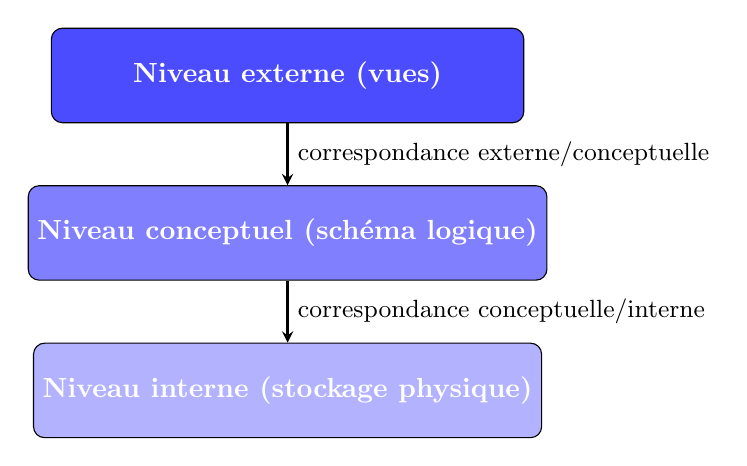
\begin{tikzpicture}[
    niveau/.style={draw, rounded corners, minimum width=6cm, minimum height=1.2cm,
                   font=\bfseries, text=white},
    fleche/.style={->, thick, >=stealth}
]
    \node[niveau, fill=blue!70] (ext) at (0,4) {Niveau externe (vues)};
    \node[niveau, fill=blue!50] (con) at (0,2) {Niveau conceptuel (sch\'ema logique)};
    \node[niveau, fill=blue!30] (int) at (0,0) {Niveau interne (stockage physique)};

    \draw[fleche] (ext) -- (con) node[midway, right, font=\small] {correspondance externe/conceptuelle};
    \draw[fleche] (con) -- (int) node[midway, right, font=\small] {correspondance conceptuelle/interne};
\end{tikzpicture}
\end{center}

\begin{theoreme}[Ind\'ependance des donn\'ees]
L'architecture trois niveaux garantit deux formes d'ind\'ependance~:
\begin{itemize}
    \item \textbf{Ind\'ependance logique}~: on peut modifier le sch\'ema conceptuel
          sans affecter les vues externes.
    \item \textbf{Ind\'ependance physique}~: on peut modifier l'organisation physique
          (ajout d'index, changement de format) sans affecter le sch\'ema conceptuel.
\end{itemize}
\end{theoreme}

\section{Le mod\`ele relationnel}

\begin{definition}[Relation]
Soit $D_1, D_2, \ldots, D_n$ des domaines (ensembles de valeurs possibles).
Une \emph{relation} $R$ de sch\'ema $R(A_1:D_1, A_2:D_2, \ldots, A_n:D_n)$
est un sous-ensemble fini du produit cart\'esien $D_1 \times D_2 \times \cdots \times D_n$.
Chaque \'el\'ement de $R$ est appel\'e un \emph{n-uplet} (ou \emph{tuple}).
\end{definition}

\begin{formules}[title=\textbf{Terminologie relationnelle vs.\ tabulaire}]
\begin{center}
\begin{tabular}{lll}
\toprule
\textbf{Mod\`ele relationnel} & \textbf{Tableau} & \textbf{SQL} \\
\midrule
Relation & Table & \texttt{TABLE} \\
Attribut & Colonne & \texttt{COLUMN} \\
Tuple (n-uplet) & Ligne & \texttt{ROW} \\
Domaine & Type de donn\'ees & \texttt{INTEGER}, \texttt{TEXT}, \ldots \\
Degr\'e & Nombre de colonnes & --- \\
Cardinalit\'e & Nombre de lignes & \texttt{COUNT(*)} \\
\bottomrule
\end{tabular}
\end{center}
\end{formules}

\begin{definition}[Cl\'e candidate et cl\'e primaire]
Soit $R$ une relation de sch\'ema $R(A_1, \ldots, A_n)$.
\begin{itemize}
    \item Une \emph{super-cl\'e} de $R$ est un sous-ensemble $K \subseteq \{A_1, \ldots, A_n\}$
          tel que pour tout couple de tuples distincts $t_1, t_2 \in R$, on a $t_1[K] \neq t_2[K]$.
    \item Une \emph{cl\'e candidate} est une super-cl\'e minimale (aucun sous-ensemble strict
          n'est lui-m\^eme super-cl\'e).
    \item La \emph{cl\'e primaire} est la cl\'e candidate choisie par le concepteur pour
          identifier de mani\`ere unique chaque tuple.
\end{itemize}
\end{definition}

\begin{exemple}
Dans la table \texttt{Etudiants}~:
\begin{itemize}
    \item $\{$\texttt{id\_etudiant}$\}$ est cl\'e candidate (et cl\'e primaire choisie).
    \item $\{$\texttt{nom}, \texttt{prenom}, \texttt{date\_naissance}$\}$ pourrait \^etre
          une cl\'e candidate si on suppose l'unicit\'e de cette combinaison.
    \item $\{$\texttt{id\_etudiant}, \texttt{nom}$\}$ est une super-cl\'e mais pas une
          cl\'e candidate (non minimale).
\end{itemize}
\end{exemple}

\begin{definition}[Cl\'e \'etrang\`ere]
Soit deux relations $R$ et $S$. Un ensemble d'attributs $FK$ de $R$ est une
\emph{cl\'e \'etrang\`ere} r\'ef\'eren\c{c}ant $S$ si, pour tout tuple $t \in R$,
$t[FK]$ est soit \texttt{NULL}, soit \'egal \`a $s[PK]$ pour un tuple $s \in S$,
o\`u $PK$ est la cl\'e primaire de $S$.
\end{definition}

\section{Langages d'un SGBD}

\subsection{DDL --- Langage de D\'efinition de Donn\'ees}

\begin{codeblock}[title=\textbf{Cr\'eation d'une table avec contraintes}]
\begin{minted}{sql}
CREATE TABLE Etudiants (
    id_etudiant  INTEGER PRIMARY KEY,
    nom          TEXT NOT NULL,
    prenom       TEXT NOT NULL,
    date_naissance DATE,
    filiere      TEXT CHECK (filiere IN ('Info', 'Maths', 'Physique')),
    UNIQUE (nom, prenom, date_naissance)
);
\end{minted}
\end{codeblock}

\subsection{DML --- Langage de Manipulation de Donn\'ees}

\begin{codeblock}[title=\textbf{Op\'erations CRUD de base}]
\begin{minted}{sql}
-- Create (insertion)
INSERT INTO Etudiants (id_etudiant, nom, prenom, filiere)
VALUES (6, 'Garcia', 'Lucie', 'Info');

-- Read (lecture)
SELECT nom, prenom FROM Etudiants WHERE filiere = 'Info';

-- Update (mise a jour)
UPDATE Etudiants SET filiere = 'Maths' WHERE id_etudiant = 6;

-- Delete (suppression)
DELETE FROM Etudiants WHERE id_etudiant = 6;
\end{minted}
\end{codeblock}

\subsection{DCL --- Langage de Contr\^ole de Donn\'ees}

\begin{codeblock}[title=\textbf{Gestion des droits (PostgreSQL)}]
\begin{minted}{sql}
-- Accorder le droit de lecture
GRANT SELECT ON Etudiants TO utilisateur_web;

-- Accorder tous les droits
GRANT ALL PRIVILEGES ON Cours TO administrateur;

-- Revoquer un droit
REVOKE DELETE ON Etudiants FROM utilisateur_web;
\end{minted}
\end{codeblock}

\section{Principaux SGBD relationnels}

\begin{center}
\begin{tabular}{llll}
\toprule
\textbf{SGBD} & \textbf{Licence} & \textbf{Usage typique} & \textbf{Particularit\'e} \\
\midrule
PostgreSQL & Open source & Entreprise, web & Tr\`es conforme SQL \\
MySQL/MariaDB & Open source & Web (LAMP) & Tr\`es r\'epandu \\
SQLite & Domaine public & Embarqu\'e, mobile & Sans serveur \\
Oracle DB & Commercial & Grande entreprise & Tr\`es performant \\
SQL Server & Commercial & Entreprise (.NET) & Int\'egration Microsoft \\
\bottomrule
\end{tabular}
\end{center}

\section{Premiers pas avec SQLite et Python}

SQLite est int\'egr\'e \`a Python via le module \texttt{sqlite3}~:

\begin{codeblock}[title=\textbf{Connexion et cr\'eation de table avec Python}]
\begin{minted}{python}
import sqlite3

# Connexion (cree le fichier si inexistant)
conn = sqlite3.connect('universite.db')
cur = conn.cursor()

# Creation de la table
cur.execute('''
    CREATE TABLE IF NOT EXISTS Etudiants (
        id_etudiant  INTEGER PRIMARY KEY,
        nom          TEXT NOT NULL,
        prenom       TEXT NOT NULL,
        date_naissance DATE,
        filiere      TEXT
    )
''')

# Insertion
cur.execute("INSERT INTO Etudiants VALUES (1, 'Bernard', 'Alice', '2004-03-15', 'Info')")
cur.execute("INSERT INTO Etudiants VALUES (2, 'Petit', 'Bob', '2003-11-22', 'Info')")

conn.commit()

# Lecture
cur.execute("SELECT * FROM Etudiants")
for row in cur.fetchall():
    print(row)

conn.close()
\end{minted}
\end{codeblock}

\begin{codeoutput}
\begin{verbatim}
(1, 'Bernard', 'Alice', '2004-03-15', 'Info')
(2, 'Petit', 'Bob', '2003-11-22', 'Info')
\end{verbatim}
\end{codeoutput}

\begin{bonnepratique}[title=\textbf{Utiliser des requ\^etes param\'etr\'ees}]
Ne jamais construire des requ\^etes SQL par concat\'enation de cha\^ines~:
cela expose aux \emph{injections SQL}. Utiliser les param\`etres \texttt{?}~:
\begin{minted}{python}
# BON : requete parametree
cur.execute("SELECT * FROM Etudiants WHERE filiere = ?", ('Info',))

# MAUVAIS : concatenation (injection SQL possible !)
# cur.execute("SELECT * FROM Etudiants WHERE filiere = '" + filiere + "'")
\end{minted}
\end{bonnepratique}

\section{Types de donn\'ees SQL}

\begin{formules}[title=\textbf{Types de donn\'ees courants}]
\begin{center}
\begin{tabular}{lll}
\toprule
\textbf{Cat\'egorie} & \textbf{Type SQL} & \textbf{Description} \\
\midrule
Entier & \texttt{INTEGER}, \texttt{SMALLINT}, \texttt{BIGINT} & Nombres entiers \\
R\'eel & \texttt{REAL}, \texttt{FLOAT}, \texttt{DOUBLE} & Nombres \`a virgule flottante \\
D\'ecimal & \texttt{NUMERIC(p,s)}, \texttt{DECIMAL} & Pr\'ecision exacte \\
Texte & \texttt{TEXT}, \texttt{VARCHAR(n)}, \texttt{CHAR(n)} & Cha\^ines de caract\`eres \\
Date/heure & \texttt{DATE}, \texttt{TIME}, \texttt{TIMESTAMP} & Temporel \\
Bool\'een & \texttt{BOOLEAN} & Vrai/faux \\
Binaire & \texttt{BLOB} & Donn\'ees binaires \\
\bottomrule
\end{tabular}
\end{center}
\end{formules}

\begin{attention}[title=\textbf{NULL n'est pas z\'ero}]
La valeur \texttt{NULL} repr\'esente l'absence de valeur. Elle est diff\'erente
de $0$, de la cha\^ine vide \texttt{''} ou de \texttt{FALSE}.
Toute comparaison avec \texttt{NULL} retourne \texttt{UNKNOWN} (logique ternaire).
On teste la nullit\'e avec \texttt{IS NULL} ou \texttt{IS NOT NULL}, jamais avec \texttt{= NULL}.
\end{attention}

\section{Contraintes d'int\'egrit\'e}

\begin{definition}[Contraintes d'int\'egrit\'e]
Les contraintes d'int\'egrit\'e sont des r\`egles qui garantissent la coh\'erence
des donn\'ees dans la base. Les principales contraintes sont~:
\begin{itemize}
    \item \texttt{PRIMARY KEY} --- identifie de mani\`ere unique chaque ligne.
    \item \texttt{FOREIGN KEY} --- r\'ef\'erence une cl\'e primaire d'une autre table.
    \item \texttt{NOT NULL} --- interdit les valeurs nulles.
    \item \texttt{UNIQUE} --- interdit les doublons.
    \item \texttt{CHECK} --- v\'erifie une condition logique.
    \item \texttt{DEFAULT} --- valeur par d\'efaut si aucune n'est fournie.
\end{itemize}
\end{definition}

\begin{codeblock}[title=\textbf{Exemple complet de contraintes}]
\begin{minted}{sql}
CREATE TABLE Inscriptions (
    id_etudiant INTEGER NOT NULL,
    id_cours    INTEGER NOT NULL,
    note        REAL CHECK (note >= 0 AND note <= 20),
    annee       INTEGER DEFAULT 2025,
    PRIMARY KEY (id_etudiant, id_cours),
    FOREIGN KEY (id_etudiant) REFERENCES Etudiants(id_etudiant)
        ON DELETE CASCADE,
    FOREIGN KEY (id_cours) REFERENCES Cours(id_cours)
        ON UPDATE CASCADE
);
\end{minted}
\end{codeblock}

\section{Mod\`eles de donn\'ees~: panorama}

Outre le mod\`ele relationnel, d'autres mod\`eles existent~:

\begin{center}
\begin{tabular}{lll}
\toprule
\textbf{Mod\`ele} & \textbf{Structure} & \textbf{Exemple de SGBD} \\
\midrule
Relationnel & Tables (lignes/colonnes) & PostgreSQL, MySQL \\
Document & Documents JSON/BSON & MongoDB, CouchDB \\
Cl\'e-valeur & Paires cl\'e $\to$ valeur & Redis, DynamoDB \\
Colonne & Familles de colonnes & Cassandra, HBase \\
Graphe & N\oe{}uds et ar\^etes & Neo4j, ArangoDB \\
\bottomrule
\end{tabular}
\end{center}

Le chapitre~\ref{ch:nosql} approfondira ces alternatives.

\section*{Exercices}

\begin{exercice}
Donnez trois avantages d'un SGBD par rapport \`a un syst\`eme de fichiers plat
(CSV). Illustrez chaque avantage avec un exemple concret li\'e \`a la gestion
d'une universit\'e.
\end{exercice}

\begin{exercice}
Pour chacune des tables suivantes, identifiez la ou les cl\'es candidates~:
\begin{enumerate}
    \item \texttt{Livres(isbn, titre, auteur, annee\_publication)}
    \item \texttt{Employes(matricule, nom, prenom, email, departement)}
    \item \texttt{Vols(compagnie, numero\_vol, date\_depart, aeroport\_depart, aeroport\_arrivee)}
\end{enumerate}
\end{exercice}

\begin{exercice}
\'Ecrivez le code SQL pour cr\'eer une base de donn\'ees de biblioth\`eque avec
les tables \texttt{Livres}, \texttt{Auteurs}, \texttt{Emprunts} et
\texttt{Adherents}. D\'efinissez les cl\'es primaires, cl\'es \'etrang\`eres
et au moins deux contraintes \texttt{CHECK}.
\end{exercice}

\begin{exercice}
\'Ecrivez un script Python utilisant \texttt{sqlite3} qui~:
\begin{enumerate}
    \item Cr\'ee la base de donn\'ees \texttt{bibliotheque.db}.
    \item Cr\'ee les tables d\'efinies \`a l'exercice pr\'ec\'edent.
    \item Ins\`ere au moins 5 livres et 3 adh\'erents.
    \item Affiche tous les livres dont l'ann\'ee de publication est sup\'erieure \`a 2020.
\end{enumerate}
\end{exercice}

\begin{exercice}
Expliquez la diff\'erence entre ind\'ependance logique et ind\'ependance physique
des donn\'ees dans l'architecture ANSI/SPARC. Donnez un exemple concret pour chaque type.
\end{exercice}
